
%----------------------------------------------------------------------------------------
%	Lecture 9
%----------------------------------------------------------------------------------------

\chapter{Second Order Linear Differential Equations} 

\bigbreak

\section{Second Order Linear Differential Equations with Constant Coefficients}

In standard form, the homogenous equation looks like,

$$ y'' + Ay' + B = 0 $$

We're going to assume that the general solution is $ y = c_1 y_1 + c_2 y_2 $ 
because since this is a second order equation so we'll have two arbitary constants.

Here, if we set $c_1 = 1$ and $c_2 = 0$ then $y_1$ is a solution to this equation.
If we set $c_1 = 0$ and $c_2 = 1$ then $y_2$ is also a solution to this equation.

Thus, to find a general solution, all we need to do is find two solutions to this equation.

The initial conditions are satisfied by choosing $c_1$ and $c_2$ properly.

\begin{figure}[ht!]
    \centering
    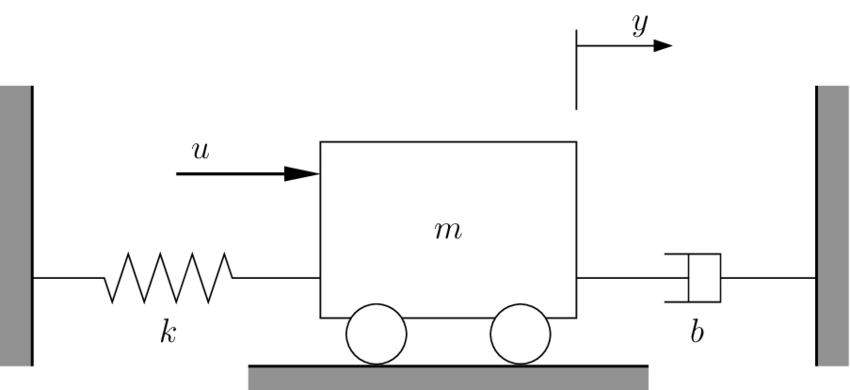
\includegraphics[scale=0.3]{./images/lecture_9_figure_1.png}
    \caption{Spring-Mass-Dashpot System}
\end{figure}

We'll take the origin at the equilibrium position.
Let's take the displacement as $x(t)$. Then the force is 

$$ ma = -kx - cv $$

The spring applies force in the opposite direction of the displacement.
The dashpot opposes motion so it applies a force opposite to the velocity.
Now, writing $a$ as $x''$ and $v$ as $x'$ and converting to its standard form, we get,

$$ x'' + \frac{c}{m}x' + \frac{k}{m}x = 0 $$


\subsection{Method to Find Solution}

To solve the above equation, we want to find two solutions.
But there is a condition that the two solutions must be independent, 
that is, the one solution must not be a constant multiple of the other.
This rules out the trivial solution of $y = 0$. 

We'll find the solution as $y = e^{rt}$ and find $r$. 
Sustituting we get,

\begin{gather*}
    r^2 e^{rt} + Ar e^{rt} + B e^{rt} = 0 \\
    \Rightarrow (r^2 + Ar + B) e^{rt} = 0
\end{gather*}

Since $e^{rt}$ is never zero so the term $r^2 + Ar + B$ must be zero. 
This is called the {\bf Characteristic Equation}.
And solving this we'll get the two values of $r$ which will give us two solution of the equation.
Now there are three cases.

{\bf Case 1 : } The roots are real and unequal.
 
Here our solution will be $y = c_1 e^{r_1 t} + c_2 e^{r_2 t}$.

{\bf Example : } $y'' + 4y' + 3 = 0$

The characteristic equation is $r^2 + 4y + 3 = 0 \Rightarrow r = -1, -3$.
So the general solution is $y = c_1 e^{-t} + c_2 e^{-3t}$.
And $y' = -c_1 e^{-t} - 3c_2 e^{-3t}$.
We have the initial condition as $y(0) = c_1 + c_2 = 1$ and $y'(0) = -c_1 - 3c_2 = 0$.
Solving there we'll get, $c_1 = \frac{3}{2}$ and $c_2 = \frac{-1}{2}$. 

So our final solution is $y(t) = \frac{3}{2}e^{-t} - \frac{1}{2} e^{-3t}$.
This solution tells us that no matter where you start, as $t \to \infty$ it goes to zero.
This case is called Overdamped.

{\bf Case 2 : } The roots are complex conjugate pair.

Here the roots are $a \pm bi$. 
We have a complex solution $y = e^{(a+bi)t}$.
Now, if you have a complex solution $u + vi$ to a real differential equation 
where $u$ and $v$ are real. Then $u$ and $v$ are real solution to the differential equation. 

So our solution $e^{at + ibt}$ have real part $e^{at}\cos(bt)$ and the imaginary part is $e^{at}\sin(bt)$.
Thus, our final solution is $e^{at}(c_1 \cos(at) + c_2 \cos(bt))$.
We can convert to $Ae^{at} \cos(bt - \phi)$ 
so this is a sinusoidal equation with an exponential amplitute.

{\bf Example : } $y'' + 4y + 5 = 0$

The characteristic equation is $r^2 + 4y + 5 = 0$ so our solution are $r = -2 + \pm t$.
So our solution is $e^{-2t}(c_1 \cos t + c_2 \sin t)$.
You can find the constants by using the initial values.
This is called Underdamped.

\begin{figure}[ht!]
    \centering
    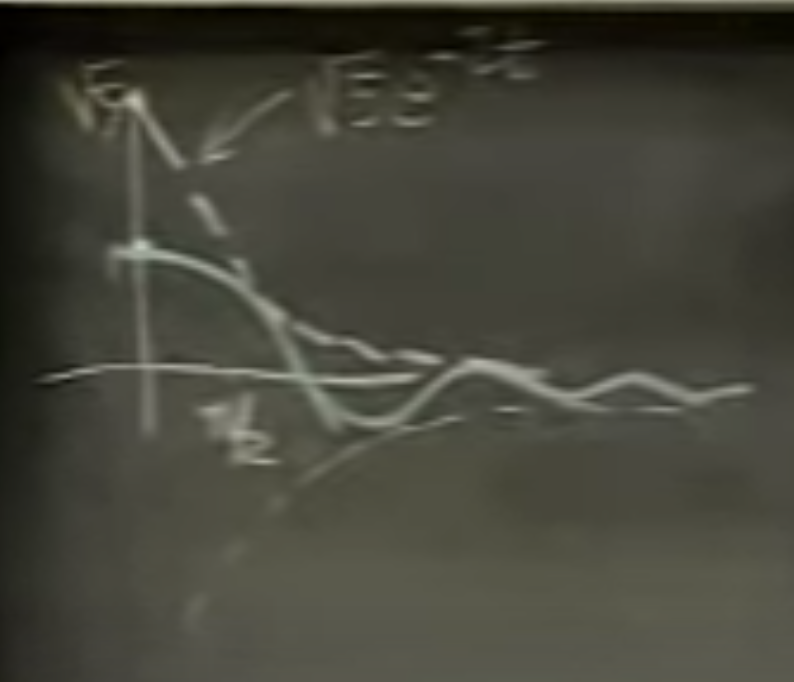
\includegraphics[scale=0.25]{./images/lecture_9_figure_2.png}
    \caption{Plot of the curve $Ae^{-2t}\cos(t - \phi)$}
\end{figure}

{\bf Case 3 : } Solutions are real and equal.

So $r^2 + Ar + B = 0$ has two equal roots.
Usually the roots are negative so we take $r = -a$.
So the characteristic equation is $(r+a)^2 = r^2 + 2ar + a^2 = 0$
So our differential equation will be $y'' + 2a y' + a^2 y = 0$

So we have only one solution $y = e^{-at}$.

Another theorem says, that if you have one solution of $y_1$ to the equation $y'' + Ay' + Qy = 0$
then there is another solution $y = y_1 u$ wher $u$ is some function.
And you will be able to find $u$.

Substituting $y = e^{-at} u$ in the original differential equation.
\begin{align*}
    y' & = -ae^{-at} u + e^{-at} u' \\
    y'' & = a^2 e^{-at} u - a e^{-at} u' -a e^{-at} u' + e^{-at} u'' \\
    y'' & = a^2 e^{-at} u - 2 a e^{-at} u' + e^{-at} u'' \\
    & y'' + 2ay' + a^2y = 0 \\
    & \Rightarrow a^2 e^{-at} u - 2 a e^{-at} u' + e^{-at} u'' \\
    & - 2 a^2 e^{-at} u + 2a e^{-at} u' \\
    & + a^2 e^{-at} u = 0 \\
    & \Rightarrow e^{-at} u'' = 0
\end{align*}
Since $e^{-at}$ is always non-zero then $u'' = 0$ so $u = (c_1t + c_2)$.
So our general solution is $y = e^{-at}(c_1t + c_2)$.
